
\documentclass[nohyperref]{article}

\usepackage{microtype}
\usepackage{graphicx}
\usepackage{subcaption}
\usepackage{booktabs} %

\usepackage{hyperref}


\newcommand{\theHalgorithm}{\arabic{algorithm}}


\usepackage[accepted]{icml2023}

\usepackage{amsmath}
\usepackage{amssymb}
\usepackage{mathtools}
\usepackage{amsthm}

\usepackage[capitalize,noabbrev]{cleveref}

\theoremstyle{plain}
\newtheorem{theorem}{Theorem}[section]
\newtheorem{proposition}[theorem]{Proposition}
\newtheorem{lemma}[theorem]{Lemma}
\newtheorem{corollary}[theorem]{Corollary}
\theoremstyle{definition}
\newtheorem{definition}[theorem]{Definition}
\newtheorem{assumption}[theorem]{Assumption}
\theoremstyle{remark}
\newtheorem{remark}[theorem]{Remark}

\usepackage[textsize=tiny]{todonotes}


\icmltitlerunning{Leveraging Task Structures for Improved Identifiability in Neural Network Representations}

\begin{document}

\twocolumn[
\icmltitle{Leveraging Task Structures for Improved Identifiability\\in Neural Network Representations}



\icmlsetsymbol{equal}{*}

\begin{icmlauthorlist}
\icmlauthor{Wenlin Chen}{equal,cambridge,mpi}
\icmlauthor{Julien Horwood}{equal,cambridge}
\icmlauthor{Juyeon Heo}{cambridge}
\icmlauthor{José Miguel Hernández-Lobato}{cambridge}

\end{icmlauthorlist}

\icmlaffiliation{cambridge}{University of Cambridge, Cambridge, United Kingdom}
\icmlaffiliation{mpi}{Max Planck Institute for Intelligent Systems, T{\"u}bingen, Germany}

\icmlcorrespondingauthor{Julien Horwood}{jdh95@cam.ac.uk}
\icmlcorrespondingauthor{Wenlin Chen}{wc337@cam.ac.uk}

\icmlkeywords{Machine Learning, ICML}

\vskip 0.3in
]



\printAffiliationsAndNotice{\icmlEqualContribution} %

\begin{abstract}
This work extends the theory of identifiability in supervised learning by considering the consequences of having access to a distribution of tasks.
In such cases, we show that identifiability is achievable even in the case of regression, extending prior work restricted to the single-task classification case.
Furthermore, we show that the existence of a task distribution which defines a conditional prior over latent variables reduces the equivalence class for
identifiability to permutations and scaling, a much stronger and more useful result. When we further assume a causal structure over these tasks, our approach
enables simple maximum marginal likelihood optimization together with downstream applicability to causal representation learning. 
Empirically, we validate that our model outperforms more general unsupervised models in recovering canonical representations for 
synthetic and real-world data.


\end{abstract}

\section{Introduction}

Multi-task regression is a common problem in machine learning, which naturally arises in many scientific applications such as molecular property prediction \citep{stanley2021fsmol,chen2023metalearning}. Despite this, most deep learning approaches to
this problem attempt to model the relationships between tasks through heuristic approaches, such as fitting a shared neural network in an attempt to capture joint structures between tasks.
Beyond lacking a principled approach to modeling task relationships, these approaches fail to account for how we may expect the latent factors for related tasks to change. In particular, a common assumption
in the causal representation learning literature, known as the sparse mechanisms shift hypothesis \citep{peters2017elements,scholkopf2019causality,scholkopf2021toward}, states that changes across tasks arise from sparse changes in the underlying causal mechanisms. Thus, it is natural
to consider the implications of such a hypothesis in the multi-task setting. In this work, we show that by leveraging assumptions about the relationships between the latent factors of the data \textit{across} 
tasks, in particular that they vary sparsely in their causal and spurious relationships, we can achieve identifiability of the latent factors up to permutations and scaling, and simultaneously identify the causal and spurious latent factors with respect to the target variable. We accomplish this by first
extending the theory of identifiability in supervised learning to the multi-task regression setting for identifiability up to linear transformations, where prior work has been restricted
to the single-task classification case. We then propose a new approach to identifying neural network representations up to permutations and scaling, by leveraging the causal structures 
of the underlying latent factors for each task. We emphasize that this is a \textit{stronger} identifiability result than identifiability up to \textit{block} permutations and scaling as in \citet{Khemakhem_Kingma_Monti_Hyvarinen_2020,Lu_Wu_Hernandez-Lobato_Scholkopf_2022}. In simulated settings where data is generated from our model, we empirically validate our model's ability to recover the true latent structure of the data. This contrasts 
with current state-of-the-art approaches, whose assumptions also fit our generative process but which are difficult to train effectively and only identifiable up to block transformation.
We also empirically validate that our model is capable of recovering canonical representations for real-world molecular data.

\section{Related Work}

The notion of optimizing for disentangled representations gained traction in the recent unsupervised deep learning literature when it was proposed that this 
objective may be sufficient to improve desirable attributes such as interpretability, robustness, and generalization \citep{Higgins_Matthey_Pal_Burgess_Glorot_Botvinick_Mohamed_Lerchner_2017,chen2016infogan}. However, 
the notion of disentanglement alone is not intrinsically well-defined, as there may be many disentangled representations of the data which are seemingly equally valid. Thus it is not clear a priori that this criterion is sufficient to
achieve the above desiderata \citep{Locatello_Bauer_Lucic_Raetsch_Gelly_Scholkopf_Bachem_2019}. In the causal representation learning literature, the \textit{correct} disentangled representation is assumed to be the one 
which corresponds to the ground-truth data generating process. Thus, what is required is an \textit{identifiable} representation, which must be equivalent to the causal one for sufficiently expressive models. In the linear case, identifiability results exist 
in the classical literature for ICA, which requires non-gaussianity assumptions on the sources for the data \citep{Herault_Jutten_1986,Comon_1994}. Extensions of ICA to the non-linear case have been proposed more recently, together with significant theoretical advances. In particular, \citet{hyvarinen2019nonlinear} extend this by assuming a conditionally factorized prior over the latent variables, and propose a contrastive learning objective for recovering the inverse of the function which generated the observations.
\citet{Khemakhem_Kingma_Monti_Hyvarinen_2020} further extend this to the setting of noisy observations, drawing connections with variational autoencoders \citep{kingma2013auto} and enabling direct optimization via a variational objective. Finally, \citet{Lu_Wu_Hernandez-Lobato_Scholkopf_2022}
derive analogous results for the case where the prior over the latent variables is a more general non-factorized exponential family distribution, while connecting the obtained causal representations to out-of-distribution prediction. However,
the complex nature of the prior requires score matching, which is difficult to optimize in practice.
While these works are generally concerned with the unsupervised and semi-supervised setting, \citet{Roeder_Metz_Kingma_2021} discuss the identifiability properties of learned representations in the case of single-task supervised classification, showing 
that the representations obtained via the final hidden layer of a neural network are identifiable up to \textit{linear} transformations, which may not be a sufficiently restrictive equivalence class for practical applicability.

\section{Proposed Method}\label{sec:proposed_method}

We propose a novel method that leverages task structures in the multi-task regression setting to identify the ground-truth data representations up to permutations and scaling, where we have access to a distribution $p(t)$ over $N_T$ training tasks $\{1,\cdots,N_T\}$.
Overall, our method consists of two stages. In the first stage, we train a multi-task neural network with a feature extractor shared across tasks and task-specific linear heads. We show that upon convergence, the representations learned by the feature extractor are identifiable up to some invertible linear transformation. In the second stage, we assume a causal structure across tasks and use it to define a conditional prior over the linearly identifiable representations obtained in the first stage. We show that this enables simple maximum marginal likelihood learning for recovering the linear transformation, which reduces the identifiability class to permutations and scaling, and automatically disentangles and identifies the causes and effects of the target variable from the learned representations. 

\subsection{Stage 1: Multi-Task Regression Network}
Let $f_{\boldsymbol{\phi},\mathbf{w}_t}(\mathbf{x})=\mathbf{w}_t^{\text{T}}\mathbf{h}_{\boldsymbol{\phi}}(\mathbf{x})$ be the output of a multi-task regression network (MTRN) for task $t$, 
where $\mathbf{w}_t\in\mathbb{R}^{D}$ are the regression weights in the linear head for task $t$, and $\mathbf{h}_{\boldsymbol{\phi}}(\mathbf{x})\in\mathbb{R}^{D}$ is the feature extractor shared across all tasks.
As in typical non-linear regression settings, 
the target variable $y\in\mathbb{R}$ is assumed to be distributed as a Gaussian $p_{\boldsymbol{\phi},\mathbf{w}}(y|\mathbf{x},t)=\mathcal{N}(y|f_{\boldsymbol{\phi},\mathbf{w}_t}(\mathbf{x}),\sigma_r^2)$ with mean modelled by the MTRN and variance fixed to some constant $\sigma_r^2$.
Denote the ground-truth predictive distribution by $p_{\boldsymbol{\phi}^*,\mathbf{w}^*}(y|\mathbf{x},t)$.
We first define linearly identifiable representations.
\begin{definition}\label{def:weak-id}
    Neural network representations are \textit{linearly identifiable} if there exists an invertible matrix $\mathbf{A}_{*}\in\mathbb{R}^{D\times D}$ such that
    \begin{equation}
        \begin{split}
            p_{\boldsymbol{\phi},\mathbf{w}}(y|\mathbf{x},t)&=p_{\boldsymbol{\phi}^*,\mathbf{w}^*}(y|\mathbf{x},t),~\forall t,\mathbf{x},y \\
            &\iff \mathbf{h}_{\boldsymbol{\phi}}(\mathbf{x})=\mathbf{A}_{*}\mathbf{h}_{\boldsymbol{\phi}^*}(\mathbf{x}).
        \end{split}
    \end{equation}
\end{definition}
We train the MTRN $f_{\boldsymbol{\phi},\mathbf{w}_t}$ using maximum likelihood:
\begin{align}
    \max_{\boldsymbol{\phi},\mathbf{w}}~\mathbb{E}_{p(t)p(\mathbf{x},y|t)}[\log p_{\boldsymbol{\phi},\mathbf{w}}(y|\mathbf{x},t)],
\end{align}
where $p(\mathbf{x},y|t)$ is the data distribution for task $t$. We show that the representations learned by the feature extractor $\mathbf{h}_{\boldsymbol{\phi}}$ of an MTRN are linearly identifiable upon convergence to the ground-truth predictive distribution, assuming that we have access to a set of sufficiently diverse tasks measured by the linear dependencies between their regression weights. 
\begin{theorem}\label{thm:lin-id}
    Suppose that there exist $D$ tasks $\{t_i\}_{i=1}^D$ such that the set of regression weights $\{\mathbf{w}_{t_i}\}_{i=1}^D$ learned by an MTRN $f_{\boldsymbol{\phi},\mathbf{w}_t}$ via maximum likelihood and the set of ground-truth regression weights $\{\mathbf{w}_{t_i}^*\}_{i=1}^D$ are two sets of linearly independent vectors.
    Let $\mathcal{H}_t\coloneqq\{p_{\boldsymbol{\phi},\mathbf{w}}(y|\mathbf{x},t)|(\boldsymbol{\phi},\mathbf{w})\in\boldsymbol{\Theta}\}$ be our hypothesis class of the predictive distribution, where $\boldsymbol{\Theta}$ is the parameter space. Assume $p_{\boldsymbol{\phi}^*,\mathbf{w}^*}(y|\mathbf{x},t)\in\mathcal{H}_t,~\forall t$. 
    Then, the representations $\mathbf{h}_{\boldsymbol{\phi}}(\mathbf{x})$ learned by the MTRN via maximum likelihood are linearly identifiable.
    \label{thm:linear-identifiability}
\end{theorem}

\begin{figure}[!ht]
    \centering
    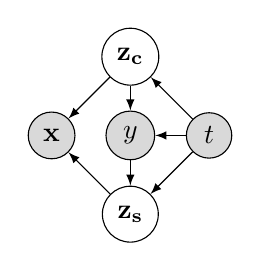
\begin{tikzpicture}[>=latex]
        \node[draw, circle, fill=gray!30] (T) at (2.5,-0.5) {$t$};
        \node[draw, circle, fill=gray!30] (X) at (0.5,-0.5) {$\mathbf{x}$};
        \node[draw, circle] (Z_c) at (1.5,0.5) {$\mathbf{z_c}$};
        \node[draw, circle] (Z_s) at (1.5,-1.5) {$\mathbf{z_s}$};
        \node[draw, circle, fill=gray!30] (Y) at (1.5,-0.5) {$y$};
    
        \draw[->] (T) -- (Z_s);
        \draw[->] (T) -- (Z_c);
        \draw[->] (T) -- (Y);
        \draw[->] (Z_s) -- (X);
        \draw[->] (Z_c) -- (X);
        \draw[->] (Z_c) -- (Y);
        \draw[->] (Y) -- (Z_s);
    \end{tikzpicture}
    \caption{Assumed causal graph for the data generating process.}
    \label{fig:causal-graph}
\end{figure}

\subsection{Stage 2: Multi-Task Linear Causal Model} 
In order to reduce the identifiability class from linear to permutations and scaling for our learned representations $\mathbf{h}_{\boldsymbol{\phi}}(\mathbf{x})$, we further assume a causal graph for the ground-truth data generating process, as shown in Figure \ref{fig:causal-graph}. We assume that the observed variable $\mathbf{x}$ is generated by some (unobserved) ground-truth data representations (or latent variables) $\mathbf{z}^*=\mathbf{h}_{\boldsymbol{\phi}^*}(\mathbf{x})$. Each task $t$ has its own partition of the latent variables into a set of causal latent variables $\mathbf{z}_c^*$ (i.e., parents of the target variable $y$) and a set of spurious latent variables $\mathbf{z}_s^*$ (i.e., children of the target variable $y$). We fix the feature extractor $\mathbf{h}_{\boldsymbol{\phi}}$ learned in the first stage and denote the linearly identifiable representations extracted from it by $\mathbf{h}\coloneqq\mathbf{h}_{\boldsymbol{\phi}}(\mathbf{x})$. Theorem \ref{thm:lin-id} suggests that $\mathbf{h}=\mathbf{A}_{*}\mathbf{z}^*$ for some invertible matrix $\mathbf{A}_{*}$.

We propose a \textit{multi-task linear causal model} (MTLCM) to recover $\mathbf{z}^*$ from $\mathbf{h}$ following our assumed causal graph. Let $\mathcal{T}(t)=\{\mathbf{c}_t,\boldsymbol{\gamma}_t,\mathbf{w}_t\}$ be a collection of task-specific variables associated with task $t$, which are free parameters to be learned from data, where $\mathbf{c}_t\in\{0,1\}^D$ are the causal indicator variables which determine the partition of $\mathbf{z}=\mathbf{z}_c\cup\mathbf{z}_s$ for the given task $t$, $\mathbf{w}_t$ are the regression weights for the causal latent variables, and $\boldsymbol{\gamma}_t$ are the coefficients used to generate the spurious latent variables from $y$. We assume that the causal latent variables $\mathbf{z}_c$ are sampled from a standard Gaussian distribution:
\begin{align}
    p(\mathbf{z}_c)=\mathcal{N}(\mathbf{z}_c|\mathbf{0},\mathbf{I}).
\end{align}
Following the settings in stage 1 that the target variable $y$ is a linear function of the data representations, we assume that $y$ is generated from $\mathbf{z}_c$ via a linear Gaussian model:
\begin{align}
    p_{\mathcal{T}}(y|\mathbf{z}_c,t) & =\mathcal{N}(y|(\mathbf{w}_t\circ\mathbf{c}_t)^{\text{T}}\mathbf{z},\sigma_{p}^{2}),
\end{align}
and that the spurious latent variables $\mathbf{z}_s$ are generated from $y$ via another linear Gaussian model:
\begin{align}
    p_{\mathcal{T}}(\mathbf{z}_s|y,t)=\mathcal{N}(\mathbf{z}_s|y\boldsymbol{\gamma}_t,\sigma_s^2\mathbf{I}).
\end{align}
Assuming an uninformative prior over $\mathbf{w}_t$, we propose a conditional prior over the latent variables that follows our assumed causal structures:
\begin{align}\label{eq:lin-causal-prior}
        p_{\mathcal{T}}(\mathbf{z}|y,t)
        =p(\mathbf{z}_c)p_{\mathcal{T}}(\mathbf{z}_s|y,t)
        =\mathcal{N}(\mathbf{z}|\mathbf{a}_t,\boldsymbol{\Lambda}_t),
\end{align}
where
\begin{align}
    \mathbf{a}_t&\coloneqq y\boldsymbol{\gamma}_t\circ(1-\mathbf{c}_t),\\
    \boldsymbol{\Lambda}_t&\coloneqq \text{diag}(\sigma_{s}^{2}(1-\mathbf{c}_t)+\mathbf{c}_t).
\end{align}
Since the linearly identifiable data representation $\mathbf{h}$ is equivalent to $\mathbf{z}^*$ up to a linear transformation, we assume a linear Gaussian likelihood with linear transformation $\mathbf{A}$:
\begin{align}\label{eq:s2-lkl}
    p_{\mathbf{A}}(\mathbf{h}|\mathbf{z}) & =\mathcal{N}(\mathbf{h}|\mathbf{A}\mathbf{z},\sigma_{o}^{2}\mathbf{I}).
\end{align}
Then, the marginal likelihood for $\mathbf{h}$ under our MTLCM is given by
\begin{align}\label{eq:s2-mlkl}
    p_{\mathbf{A},\mathcal{T}}(\mathbf{h}|y,t)=\int p_{\mathbf{A}}(\mathbf{h}|\mathbf{z})p_{\mathcal{T}}(\mathbf{z}|y,t)d\mathbf{z}
    =\mathcal{N}(\mathbf{h}|\boldsymbol{\mu}_t,\boldsymbol{\Sigma}_t),
\end{align}
where
\begin{align}
    \boldsymbol{\mu}_t &= y\mathbf{A}\boldsymbol{\gamma}_t\circ(1-\mathbf{c}_t),\\
    \boldsymbol{\Sigma}_t &= \mathbf{A}\text{diag}(\sigma_{s}^{2}(1-\mathbf{c}_t)+\mathbf{c}_t)\mathbf{A}^{\text{T}}+\sigma_o^2\mathbf{I}.
\end{align}
It is worth noting that in the single-task setting, the conditional prior $p(\mathbf{z}|y)$ over the latent variables $\mathbf{z}$ is non-factorized. This is because the causal latent variables $\mathbf{z}_c$ are parents of the target variable $y$, which become correlated when conditioning on $y$. In order to guarantee strong identifiability, \citet{Lu_Wu_Hernandez-Lobato_Scholkopf_2022} propose to model such non-factorized conditional priors using energy-based models, which turns out to be difficult to learn in practice. In contrast, by conditioning on the task $t$ in addition to the target $y$ and leveraging the change in the causal/spurious latent factors across tasks, we obtain a conditionally factorized prior \eqref{eq:lin-causal-prior}, which, together with the linear Gaussian likelihood \eqref{eq:s2-lkl}, allows us to use maximum marginal likelihood
\begin{align}
    \max_{\mathbf{A},\mathcal{T}}~\mathbb{E}_{p(t)p(\mathbf{x},y|t)}[\log p_{\mathbf{A},\mathcal{T}}(\mathbf{h}_{\boldsymbol{\phi}}(\mathbf{x})|y,t)]
\end{align}
to recover the ground-truth latent variables $\mathbf{z}^*$ up to permutations and scaling from the linearly identifiable data representations $\mathbf{h}=\mathbf{h}_{\boldsymbol{\phi}}(\mathbf{x})$ learned in the first stage.

Denote $\mathcal{T}_{*}(t)$ the ground-truth task-specific variables for task $t$ and $\mathbf{u}\coloneqq[y,t]$ the conditioning variable. Let $k\coloneqq2D$. We first define identifiable latent variables up to permutation and scaling and show the identifiability result of MTLCM.
\begin{definition}\label{def:strong-id}
    The latent variables are identifiable up to permutation and scaling if there exists a permutation and scaling matrix $\mathbf{P}\in\mathbb{R}^{D\times D}$ 
    such that 
    \begin{equation}
        \begin{split}
            p_{\mathbf{A},\mathcal{T}}(\mathbf{h}|\mathbf{u})=p_{\mathbf{A}_{*},\mathcal{T}_{*}}(\mathbf{h}|\mathbf{u})
            &\iff\mathbf{A}^{-1}\mathbf{h}=\mathbf{P}(\mathbf{A}_*^{-1}\mathbf{h})\\
            &\iff\mathbf{z}=\mathbf{P}\mathbf{z}^*.
        \end{split}
    \end{equation}
    We emphasize that this identifiability class is \textit{stronger} than the identifiability class up to \textit{block} permutations and scaling as in \citet{Khemakhem_Kingma_Monti_Hyvarinen_2020,Lu_Wu_Hernandez-Lobato_Scholkopf_2022}:
    \begin{align}
        \mathbf{T}(\mathbf{z})=\mathbf{P}_b\mathbf{T}_*(\mathbf{z}^*)+\mathbf{b},
    \end{align}
    where each block $i$ in the block matrix $\mathbf{P}_b$ transforms all elements that are functions of $z_i$ between the sufficient statistics $\mathbf{T}$ and $\mathbf{T}_*$ of the conditional prior, and $\mathbf{b}$ is a vector.
\end{definition}
We show that the latent variables of MTLCM are identifiable up to permutation and scaling as defined by Definition \ref{def:strong-id}.
\begin{theorem}\label{thm:lin-causal-id}
    Assume that $\mathbf{A}$ and $\mathbf{A}_{*}$ are invertible, and there exist $k+1$ points $\mathbf{u}_0, \mathbf{u}_1,\cdots,\mathbf{u}_{k}$ such that the matrix
    \begin{align}
        \mathbf{L}\coloneqq[\boldsymbol{\eta}(\mathbf{u}_1)-\boldsymbol{\eta}(\mathbf{u}_0),\cdots,\boldsymbol{\eta}(\mathbf{u}_{k})-\boldsymbol{\eta}(\mathbf{u}_0)]
    \end{align}
    is invertible, where $\boldsymbol{\eta}(\mathbf{u})\coloneqq\left[\begin{smallmatrix}\boldsymbol{\Lambda}_t^{-1}\mathbf{a}_t \\ -\frac{1}{2}\text{diag}(\boldsymbol{\Lambda}_t)\end{smallmatrix}\right]\in\mathbb{R}^{k}$ are the natural parameters of $p_{\mathcal{T}}(\mathbf{z}|\mathbf{u})$. Then, the latent variables $\mathbf{z}$ learned by the MTLCM via maximum marginal likelihood are identifiable up to permutations and scaling.
\end{theorem}

\begin{figure*}[ht]
    \centering
    \begin{subfigure}[t]{0.3\linewidth}
        \centering
        \includegraphics[width=\linewidth]{Figures/synthetic_linear_ablation.pdf}
        \caption{Scalability of MTLCM.}
        \label{fig:linear-synthetic-ablation}
    \end{subfigure}
    \hfill
    \begin{subfigure}[t]{0.65\linewidth}
        \includegraphics[width=\linewidth]{Figures/linear_methods_plot.pdf}
        \caption{Comparison across identifiable models.}
        \label{fig:linear-methods-comparison}
    \end{subfigure}
    \caption{Identifiability performance for linearly transformed synthetic latent variables. $\text{Observation Dim}=\text{Latent Dim}$.}
\end{figure*}
\begin{figure*}[!ht]
    \centering
    \includegraphics[width=\linewidth]{Figures/nonlinear_plot_comparison.pdf}
    \caption{Identifiability performance for non-linearly transformed synthetic latent variables. $\text{Latent Dim}=\min\{20,\text{Observation Dim}/2\}$.}
    \label{fig:multitask-ablation}
\end{figure*}

\section{Experiments}\label{sec:experiments}
This section empirically validates our model's ability to recover canonical representations up to permutations and scaling for 
both synthetic and real-world data. 
We contrast our model with the more general identifiable models of iVAE \citep{Khemakhem_Kingma_Monti_Hyvarinen_2020} and iCaRL \citep{Lu_Wu_Hernandez-Lobato_Scholkopf_2022}. For a fair comparison, we also consider the multi-task variations of iVAE and iCaRL, where we include the task variable $t$ in conditioning variables $\mathbf{u}$ for their conditional priors $p_{\mathcal{T}}(\mathbf{z}|\mathbf{u})$, with the task-specific free parameter $\mathcal{T}(t)=\{\mathbf{v}_t\}$ to be learned from data, which is the counterpart to $\mathcal{T}(t)=\{\mathbf{c}_t,\boldsymbol{\gamma}_t\}$ in our MTLCM but has no explicit interpretations with respect to a causal graph. 

\subsection{Synthetic Data}
We first validate our approach in the straightforward situation when the data generating process 
agrees with the assumptions of our models. For each task, we first sample the causal indicator variables $\mathbf{c}_t^*$. The causal latent factors $\mathbf{z}_c^*$ are then sampled from a standard Gaussian prior. These are then linearly combined according to random weights $\mathbf{w}_t^*$ to produced observed 
targets $y$ with a task-dependent noise corruption. Finally, the spurious variables $\mathbf{z}_s^*$ are generated via different weightings $\boldsymbol{\gamma}_t^*$ of the target $y$. This mirrors the causal data generating process described in Section \ref{sec:proposed_method}. In Section \ref{sec:linear-experiment}, we generate
observed data using random linear transformations of the ground-truth latent factors. 
In Section \ref{sec:nonlinear-experiment}, we extend this to non-linear transformations parameterized by random neural networks and demonstrate that our approach can be combined with 
the multi-task identifiability result up to linear transformations to recover permutations and scaling of the ground-truth.
We also compare the learned causal indicator variables $\mathbf{c}_t$ with the ground-truth $\mathbf{c}_t^{*}$ and results from the pair-wise conditional independence test \citep{chen2021causal,Lu_Wu_Hernandez-Lobato_Scholkopf_2022} performed on the latent variables $\mathbf{z}$ recovered by our model.

\subsubsection{Linear Case}\label{sec:linear-experiment}
We study the ability of our proposed multi-task linear causal model (MTLCM) to recover the latent variables up to permutations and scaling via the Mean Correlation Coefficient (MCC) as in \citet{Khemakhem_Kingma_Monti_Hyvarinen_2020}. The synthetic data is generated by sampling 200 tasks of 100 samples each. Each task
varies in its causal indicator variables $\mathbf{c}_t^*$, causal weights $\mathbf{w}_t^*$, and spurious coefficients $\boldsymbol{\gamma}_t^*$. We then transform the ground-truth latent variables $\mathbf{z}^*$ with a random invertible matrix $\mathbf{A}_*$ shared across all tasks to obtain linearly identifiable representations $\mathbf{h}$.
The detailed settings for these experiments can be found in Appendix \ref{appendix:experiment-settings}.
In Figures \ref{fig:linear-synthetic-ablation} and \ref{fig:linear-methods-comparison}, we show that our MTLCM manages to recover the ground-truth latent variables from $\mathbf{h}$ up to permutations and scaling, and the result is scalable as the number of latent factors and the number of causal factors increase. In contrast, iVAE, iCaRL and their multi-task variations (all with linear decoders) underperform our model by a large margin in most cases.
We also find that for all tasks, the learned causal indicator variables exactly match the ground-truth and the causal discovery results from the pair-wise conditional independence test.

\subsubsection{Non-Linear Case}\label{sec:nonlinear-experiment}
A more general analysis of the identifiability of our proposed approach is to consider the extension of the linear experiments to the setting of \textit{arbitrary} transformations of the latent variables. For this, we consider the case where random (non-linear) MLP neural networks are used to transform $\mathbf{z}^*$ into higher dimensional observations $\mathbf{x}$.
By Theorem \ref{thm:linear-identifiability}, it is possible to recover linearly identifiable representations $\mathbf{h}$ of the data by training standard MTRNs. Identifiability in this setting is assessed by first 
performing a Canonical Correlation Analysis (CCA) as in \citet{Roeder_Metz_Kingma_2021}, which linearly maps the obtained representations such that they maximize the covariance with the ground-truth latent variables. The resulting mapped representations can thus be 
compared with the ground-truth latent variables via the MCC score. 
This is referred to as weak MCC, which quantifies the linear identifiability of the learned representations from MTRNs.
We further train our MTLCM on the linearly identifiable representations $\mathbf{h}$ obtained from the MTRN to obtain identifiable representations up to permutations and scaling. Identifiability in this setting is assessed by directly computing the MCC score between the representations obtained from our MTLCM and the ground-truth latent variables as in Section \ref{sec:linear-experiment}, which is referred to as strong MCC.
We assess this for various dimensionalities of the observed data
and for different settings of the causal variables, where we generate 500 tasks of 200 samples each to improve convergence of the multitask model. The latent dimensions and hidden dimensions of the neural networks are set according to fixed heuristics, which are detailed in Appendix \ref{appendix:experiment-settings}.
In Figure \ref{fig:multitask-ablation}, we find that the strong MCC for our MTLCM is able to match or even exceed the weak MCC for the MTRN.
In contrast, the strong MCC for iVAE, iCaRL and their multi-task variations significantly underperform MTLCM. Again, we find that for all tasks, the learned causal indicator variables exactly match the ground-truth and the causal discovery results from the pair-wise conditional independence test.

\subsection{Molecular Data}
We further evaluate our model on a real-world superconductivity dataset \citep{hamidieh2018super}, which consists of $21,263$ superconductors. We consider the tasks of regressing $80$ features (excluding a trivial feature of atom count) of the superconductors from their chemical formulae. We assume that the chemical formula $\mathbf{x}$ of each superconductor is generated by transforming some unknown ground-truth latent variables $\mathbf{z}^*$ with some unknown non-linear function. Since $\mathbf{z}^*$ are unknown to us, identifiability in this setting is assessed by first training a model 5 times with different random seeds and initializations then computing the MCC score between the latent variables $\mathbf{z}$ recovered by each pair of those 5 models, as in \citet{khemakhem2020ice}.

\begin{figure}[!ht]
    \centering
    \includegraphics[width=\linewidth]{Figures/superconductivity_plot_comparison.pdf}
    \caption{Identifiability performance for the latent variables of the superconductors from the superconductivity dataset.}
    \label{fig:superconductivity}
\end{figure}

As in Section \ref{sec:nonlinear-experiment}, we use the weak MCC score to assess the linear identifiability of the representations $\mathbf{h}$ learned by the MTRN, and use the strong MCC score to assess the strong identifiability (up to permutations and scaling) of the latent variables $\mathbf{z}$ recovered by our MTLCM and the baselines (iVAE, iCaRL and their multi-task variations). In Figure \ref{fig:superconductivity}, we find that the strong MCC for our MTLCM is greater than $0.96$ and is able to match the weak MCC for the MTRN when the dimensions of the latent representations are 5 and 10. This shows that our method manages to recover canonical latent representations for the superconductors. In sharp contrast, all baseline models fail to recover identifiable latent variables for the superconductors in all cases as their strong MCC scores do not exceed $0.4$.


\section{Conclusion}
In summary, we have proposed a novel perspective on the problem of identifiable representations by exploring the implications of explicitly modeling task structures. We have shown that this 
implies new identifiability results, in particular for linear equivalence classes in the general case of multi-task regression. Furthermore, while spurious correlations have been shown to be a
failure case of deep learning in many recent works, we have demonstrated that such latent spurious signals may in fact be leveraged to \textit{improve} the ability of a model to recover more robust disentangled 
representations. In particular, we have shown that when the latent space is explicitly represented as consisting of a partitioning of causal and spurious features, the linear identifiability result
of the multi-task setting may be reduced to identifiability up to simple permutations and scaling. Finally, we have confirmed that the theoretical results hold both for the synthetic data where our model's assumptions are satisfied and for a real-world molecular dataset of superconductors. 
We anticipate that this may reveal new research directions for the study of both causal representations and synergies with 
multi-task and meta-learning methods.

\clearpage

\section*{Acknowledgements and Disclosure of Funding}
We thank Jon Paul Janet and Dino Oglic for helpful discussions. WC acknowledges funding via a Cambridge Trust Scholarship (supported by the Cambridge Trust) and a Cambridge University Engineering Department Studentship (under grant G105682 NMZR/089 supported by Huawei R\&D UK). JH acknowledges funding via a Cambridge Center for AI in Medicine Studentship (supported by AstraZeneca). JMHL acknowledges support from a Turing AI Fellowship under grant EP/V023756/1.

Part of this work was performed using resources provided by the Cambridge Service for Data Driven Discovery (CSD3) operated by the University of Cambridge Research Computing Service (\url{www.csd3.cam.ac.uk}), provided by Dell EMC and Intel using Tier-2 funding from the Engineering and Physical Sciences Research Council (capital grant EP/T022159/1), and DiRAC funding from the Science and Technology Facilities Council (\url{www.dirac.ac.uk}).

\bibliography{causal_identifiability}
\bibliographystyle{icml2023}


\newpage
\appendix
\onecolumn


\section{Proof of Theorem \ref{thm:lin-id}}\label{appendix:proof-lin-id}
\begin{proof}
    Suppose that we have trained the multi-task regression network (MTRN) $f_{\boldsymbol{\phi},\mathbf{w}_t}$ such that it has converged to the ground-truth predictive distribution:
    \begin{align}
        p_{\boldsymbol{\phi},\mathbf{w}}(y|\mathbf{x},t)&=p_{\boldsymbol{\phi}^*,\mathbf{w}^*}(y|\mathbf{x},t),\quad\forall t,\mathbf{x},y,\\
        \iff\mathcal{N}(y|f_{\boldsymbol{\phi},\mathbf{w}_t}(\mathbf{x}),\sigma_r^2) &= \mathcal{N}(y|f_{\boldsymbol{\phi}^*,\mathbf{w}_t^*}(\mathbf{x}),\sigma_r^2),\quad\forall t,\mathbf{x},y,\\
        \iff \mathcal{N}(y|\mathbf{h}_{\boldsymbol{\phi}}(\mathbf{x})^{\text{T}}\mathbf{w}_{t},\sigma_r^2) &= \mathcal{N}(y|\mathbf{h}_{\boldsymbol{\phi}^*}(\mathbf{x})^{\text{T}}\mathbf{w}_{t}^*,\sigma_r^2),\quad\forall t,\mathbf{x},y.
    \end{align}
    This implies that the means of the two Gaussian likelihoods on both sides are identical:
    \begin{align}
        \mathbf{h}_{\boldsymbol{\phi}}(\mathbf{x})^{\text{T}}\mathbf{w}_{t} &= \mathbf{h}_{\boldsymbol{\phi}^*}(\mathbf{x})^{\text{T}}\mathbf{w}_t^{*},\quad\forall t,\mathbf{x},y.\label{eq:lin-id-single}
    \end{align}
    By assumption, there exist $D$ pairs of learned and ground-truth regression weights $\{(\mathbf{w}_{t_i},\mathbf{w}_{t_i}^*)\}_{i=1}^D$ such that $\{\mathbf{w}_{t_i}\}_{i=1}^D$ and $\{\mathbf{w}_{t_i}^*\}_{i=1}^D$ are two sets of linearly independent vectors. We can thus construct two invertible matrices $\mathbf{W}=[\mathbf{w}_{t_1},\cdots,\mathbf{w}_{t_D}]\in\mathbb{R}^{D\times D}$ and $\mathbf{W}_{*}=[\mathbf{w}_{t_1}^*,\cdots,\mathbf{w}_{t_D}^*]\in\mathbb{R}^{D\times D}$. Evaluating Equation \eqref{eq:lin-id-single} at tasks $t_1,\cdots,t_D$ and stack them into matrix-vector form gives
    \begin{align}
        \mathbf{W}^{\text{T}}\mathbf{h}_{\boldsymbol{\phi}}(\mathbf{x})&=\mathbf{W}_{*}^{\text{T}}\mathbf{h}_{\boldsymbol{\phi}^*}(\mathbf{x}),\\
        \iff \quad\quad\mathbf{h}_{\boldsymbol{\phi}}(\mathbf{x})&=\mathbf{W}^{-\text{T}}\mathbf{W}_{*}^{\text{T}}\mathbf{h}_{\boldsymbol{\phi}^*}(\mathbf{x}).
    \end{align}
    Note that $\mathbf{A}_{*}\coloneqq\mathbf{W}^{-\text{T}}\mathbf{W}_{*}^{\text{T}}$ is invertible by definition. This completes the proof.
\end{proof}

\section{Proof of Theorem \ref{thm:lin-causal-id}}\label{appendix:proof-causal-id}
\begin{proof}
    Let $k\coloneqq2D$ and $\mathbf{u}\coloneqq[y,t]$. We first rewrite the density of the conditional prior in the exponential family form:
    \begin{align}
        p_{\mathcal{T}}(\mathbf{z}|\mathbf{u}) = Z(\mathbf{u})^{-1}\exp\left(\mathbf{T}(\mathbf{z})^{\text{T}}\boldsymbol{\eta}(\mathbf{u})\right),
    \end{align}
    where $Z(\mathbf{u})=(2\pi)^{D/2}|\boldsymbol{\Lambda}_t|^{0.5}\exp\left(-\frac{1}{2}\mathbf{a}_t^{\text{T}}\boldsymbol{\Lambda}_t\mathbf{a}_t\right)$ is the normalizing constant, $\mathbf{T}(\mathbf{z})=\left[\begin{smallmatrix}\mathbf{z} \\ \mathbf{z}\circ\mathbf{z}\end{smallmatrix}\right]\in\mathbb{R}^{k}$ are the sufficient statistics, and $\boldsymbol{\eta}(\mathbf{u})=\left[\begin{smallmatrix}\boldsymbol{\Lambda}_t^{-1}\mathbf{a}_t \\ -\frac{1}{2}\text{diag}(\boldsymbol{\Lambda}_t)\end{smallmatrix}\right]\in\mathbb{R}^{k}$ are the natural parameters. We also rewrite the likelihood $p_{\mathbf{A}}(\mathbf{h}|\mathbf{z})$ using the noise distribution $p_{\boldsymbol{\epsilon}_o}(\boldsymbol{\epsilon}_o)=\mathcal{N}(\boldsymbol{\epsilon}_o|\mathbf{0},\sigma_o^2\mathbf{I})$:
    \begin{align}
        p_{\mathbf{A}}(\mathbf{h}|\mathbf{z}) =\mathcal{N}(\mathbf{h}|\mathbf{A}\mathbf{z},\sigma_{o}^{2}\mathbf{I})=\mathcal{N}(\mathbf{h}-\mathbf{A}\mathbf{z}|\mathbf{0},\sigma_o^2\mathbf{I})=p_{\boldsymbol{\epsilon}_o}(\mathbf{h}-\mathbf{A}\mathbf{z}).
    \end{align}
    Let $\mathbf{A}_{*}$ be the ground-truth transformation matrix such that $\mathbf{z}^*=\mathbf{A}_{*}^{-1}\mathbf{h}$, and $\mathcal{T}_{*}(t)=\{\mathbf{c}_t^*,\boldsymbol{\gamma}_t^*\}$ the ground-truth task-specific variables associated with each task $t$. The proof starts off by using the fact that we have maximized the marginal likelihood \eqref{eq:s2-mlkl} of $\mathbf{A}$ and $\mathcal{T}$ for all tasks. This means that the marginal likelihoods of the two models are identical:
    \begin{align}\label{eq:equal-mlkl}
        p_{\mathbf{A},\mathcal{T}}(\mathbf{h}|\mathbf{u})=p_{\mathbf{A}_{*},\mathcal{T}_{*}}(\mathbf{h}|\mathbf{u}).
    \end{align}
    The goal is to show that the latent variables $\mathbf{z}=\mathbf{A}^{-1}\mathbf{h}$ recovered by our model and the ground-truth latent variable $\mathbf{z}^*=\mathbf{A}_{*}^{-1}\mathbf{h}$ are identical up to permutations and scaling for all $\mathbf{h}$. 
    
    Starting from the equality of the two marginal likelihoods \eqref{eq:equal-mlkl}, we have
    \begin{align}
        p_{\mathbf{A}}(\mathbf{h}|\mathbf{u})&=p_{\mathbf{A}_{*}}(\mathbf{h}|\mathbf{u})\\   
        \iff \int p_{\mathbf{A}}(\mathbf{h}|\mathbf{z})p_{\mathcal{T}}(\mathbf{z}|\mathbf{u})d\mathbf{z} &= \int p_{\mathbf{A}_{*}}(\mathbf{h}|\mathbf{z})p_{\mathcal{T}_{*}}(\mathbf{z}|\mathbf{u})d\mathbf{z}\\
        \iff \int p_{\boldsymbol{\epsilon}_o}(\mathbf{h}-\mathbf{A}\mathbf{z})p_{\mathcal{T}}(\mathbf{z}|\mathbf{u})d\mathbf{z} &= \int p_{\boldsymbol{\epsilon}_o}(\mathbf{h}-\mathbf{A}_{*}\mathbf{z})p_{\mathcal{T}_{*}}(\mathbf{z}|\mathbf{u})d\mathbf{z}\\
        \iff \int p_{\boldsymbol{\epsilon}_o}(\mathbf{h}-\Bar{\mathbf{h}})p_{\mathcal{T}}(\mathbf{A}^{-1}\Bar{\mathbf{h}}|\mathbf{u})\det(\mathbf{A})^{-1}d\Bar{\mathbf{h}} &= \int p_{\boldsymbol{\epsilon}_o}(\mathbf{h}-\Hat{\mathbf{h}})p_{\mathcal{T}_{*}}(\mathbf{A}_{*}^{-1}\Hat{\mathbf{h}}|\mathbf{u})\det(\mathbf{A}_{*})^{-1}d\Hat{\mathbf{h}}\label{eq:reduce-1}\\
        \iff \int p_{\boldsymbol{\epsilon}_o}(\mathbf{h}-\Bar{\mathbf{h}})\Tilde{p}_{\mathbf{A},\mathcal{T},\mathbf{u}}(\Bar{\mathbf{h}})d\Bar{\mathbf{h}} &= \int p_{\boldsymbol{\epsilon}_o}(\mathbf{h}-\Hat{\mathbf{h}})\Tilde{p}_{\mathbf{A}_{*},\mathcal{T}_{*},\mathbf{u}}(\Hat{\mathbf{h}})d\Hat{\mathbf{h}}\label{eq:reduce-2}\\
        \iff (p_{\boldsymbol{\epsilon}_o}*\Tilde{p}_{\mathbf{A},\mathcal{T},\mathbf{u}})(\mathbf{h})&=(p_{\boldsymbol{\epsilon}_o}*\Tilde{p}_{\mathbf{A}_{*},\mathcal{T}_{*},\mathbf{u}})(\mathbf{h})\label{eq:reduce-3}\\
        \iff F[p_{\boldsymbol{\epsilon}_o}](\boldsymbol{\omega})F[\Tilde{p}_{\mathbf{A},\mathcal{T},\mathbf{u}}](\boldsymbol{\omega})&=F[p_{\boldsymbol{\epsilon}_o}](\boldsymbol{\omega})F[\Tilde{p}_{\mathbf{A}_{*},\mathcal{T}_{*},\mathbf{u}}](\boldsymbol{\omega})\label{eq:reduce-4}\\
        \iff F[\Tilde{p}_{\mathbf{A},\mathcal{T},\mathbf{u}}](\boldsymbol{\omega})&=F[\Tilde{p}_{\mathbf{A}_{*},\mathcal{T}_{*},\mathbf{u}}](\boldsymbol{\omega})\label{eq:reduce-5}\\
        \iff \Tilde{p}_{\mathbf{A},\mathcal{T},\mathbf{u}}(\mathbf{h}) &= \Tilde{p}_{\mathbf{A}_{*},\mathcal{T}_{*},\mathbf{u}}(\mathbf{h})\\
        \iff p_{\mathcal{T}}(\mathbf{A}^{-1}\mathbf{h}|\mathbf{u})\det(\mathbf{A})^{-1} &= p_{\mathcal{T}_{*}}(\mathbf{A}_{*}^{-1}\mathbf{h}|\mathbf{u})\det(\mathbf{A}_{*})^{-1}\\
        \iff \mathbf{T}(\mathbf{A}^{-1}\mathbf{h})^{\text{T}}\boldsymbol{\eta}(\mathbf{u})-\log Z(\mathbf{u})-\log\det(\mathbf{A}) &= \mathbf{T}(\mathbf{A}_{*}^{-1}\mathbf{h})^{\text{T}}\boldsymbol{\eta}_{*}(\mathbf{u})-\log Z_*(\mathbf{u})-\log\det(\mathbf{A}_{*}),\label{eq:reduce-final}
    \end{align}
    where
    \begin{itemize}
        \item Equation \eqref{eq:reduce-1} follows by the definition $\Bar{\mathbf{h}}\coloneqq\mathbf{A}\mathbf{h},\Hat{\mathbf{h}}\coloneqq\mathbf{A}_{*}\mathbf{z}$,
        \item Equation \eqref{eq:reduce-2} follows by the definition $\Tilde{p}_{\mathbf{A},\mathcal{T},\mathbf{u}}(\Bar{\mathbf{h}})\coloneqq p_{\mathcal{T}}(\mathbf{A}^{-1}\Bar{\mathbf{h}}|\mathbf{u})\det(\mathbf{A})^{-1}$,
        \item $*$ in Equation \eqref{eq:reduce-3} denotes the convolution operator,
        \item $F$ in Equation \eqref{eq:reduce-4} denotes the Fourier transform operator,
        \item Equation \eqref{eq:reduce-5} follows since the characteristic function $F[p_{\boldsymbol{\epsilon}_o}]$ of the Gaussian noise $\boldsymbol{\epsilon}_o$ is nonzero almost everywhere.
    \end{itemize}
    Now we evaluate Equation \ref{eq:reduce-final} at $\mathbf{u}=\mathbf{u}_0,\mathbf{u}_1,\cdots,\mathbf{u}_k$ from our assumption to obtain $k+1$ such equations, and subtract the first equation from the remaining $k$ equations to obtain the following $k$ equations:
    \begin{align}
        \mathbf{T}(\mathbf{A}^{-1}\mathbf{h})^{\text{T}}(\boldsymbol{\eta}(\mathbf{u}_l)-\boldsymbol{\eta}(\mathbf{u}_0))+\log \frac{Z(\mathbf{u}_0)}{Z(\mathbf{u}_l)} &= \mathbf{T}(\mathbf{A}_{*}^{-1}\mathbf{h})^{\text{T}}(\boldsymbol{\eta}_{*}(\mathbf{u}_l)-\boldsymbol{\eta}_{*}(\mathbf{u}_0))+\log \frac{Z_*(\mathbf{u}_0)}{Z_*(\mathbf{u}_l)},\quad l=1,\cdots,k.
    \end{align}
    Putting those $k$ equations in matrix-vector form gives
    \begin{align}
        \mathbf{L}^{\text{T}}\mathbf{T}(\mathbf{A}^{-1}\mathbf{h})=\mathbf{L}_{*}^{\text{T}}\mathbf{T}(\mathbf{A}_{*}^{-1}\mathbf{h}) +\mathbf{q},\label{eq:ivae-lin-wip}
    \end{align}
    where $q_l=\log \frac{Z_*(\mathbf{u}_0)Z(\mathbf{u}_l)}{Z_*(\mathbf{u}_l)Z(\mathbf{u}_0)}$, $\mathbf{L}$ is the invertible matrix defined in the assumption, and $\mathbf{L}_{*}$ is similarly defined for the second model. Since $\mathbf{L}$ is invertible, we can left multiply Equation \eqref{eq:ivae-lin-wip} by $\mathbf{L}^{-\text{T}}$ to obtain
    \begin{align}
        \mathbf{T}(\mathbf{A}^{-1}\mathbf{h})=\mathbf{M}\mathbf{T}(\mathbf{A}_{*}^{-1}\mathbf{h}) +\mathbf{r},\label{eq:ivae-lin-wip-2}
    \end{align}
    where $\mathbf{M}=\mathbf{L}^{-\text{T}}\mathbf{L}_{*}^{\text{T}}$ and $\mathbf{r}=\mathbf{L}^{-\text{T}}\mathbf{q}$. We note that our assumption only says $\mathbf{L}$ is invertible and tells us nothing about $\mathbf{L}_{*}$. Therefore, we need to show that $\mathbf{M}$ is invertible.
    Let $\mathbf{h}_l\coloneqq\mathbf{A}\mathbf{z}_l,~l=0,\cdots,k$. We evaluate Equation \eqref{eq:ivae-lin-wip-2} at these $k+1$ points to obtain $k+1$ such equations, and subtract the first equation from the remaining $k$ equations. This gives us
    \begin{align}
        [\mathbf{T}(\mathbf{z}_1)-\mathbf{T}(\mathbf{z}_0),\cdots,\mathbf{T}(\mathbf{z}_k)-\mathbf{T}(\mathbf{z}_0)]=\mathbf{M}[\mathbf{T}(\mathbf{A}_{*}^{-1}\mathbf{h}_1)-\mathbf{T}(\mathbf{A}_{*}^{-1}\mathbf{h}_0),\cdots,\mathbf{T}(\mathbf{A}_{*}^{-1}\mathbf{h}_k)-\mathbf{T}(\mathbf{A}_{*}^{-1}\mathbf{h}_0)].\label{eq:ivae-lin-wip-3}
    \end{align}
    We denote Equation \eqref{eq:ivae-lin-wip-3} by $\mathbf{R}\coloneqq\mathbf{M}\mathbf{R}_{*}$. We need to show that for any given $\mathbf{z}_0$, there exist $k$ points $\mathbf{z}_1,\cdots,\mathbf{z}_k$ such that the columns of $\mathbf{R}$ are linearly independent. Suppose, for contradiction, that the columns of $\mathbf{R}$ would never be linearly independent for any $\mathbf{z}_1,\cdots,\mathbf{z}_k$. Then the function $\mathbf{g}(\mathbf{z})\coloneqq\mathbf{T}(\mathbf{z})-\mathbf{T}(\mathbf{z}_0)$ would live in a $k-1$ or lower dimensional subspace, and therefore we would be able to find a non-zero vector $\boldsymbol{\lambda}\in\mathbb{R}^k$ orthogonal to that subspace. This would imply that $(\mathbf{T}(\mathbf{z})-\mathbf{T}(\mathbf{z}_0))^{\text{T}}\boldsymbol{\lambda}=\mathbf{0}$ and thus $\mathbf{T}(\mathbf{z})^{\text{T}}\boldsymbol{\lambda}=\mathbf{T}(\mathbf{z}_0)^{\text{T}}\boldsymbol{\lambda}=const,~\forall\mathbf{z}$, which contradicts the fact that our conditionally factorized multivariate Gaussian prior $p_{\mathcal{T}}(\mathbf{z}|\mathbf{u})$ is strongly exponential (see \citet{Khemakhem_Kingma_Monti_Hyvarinen_2020} for the definition). This shows that there exist $k$ points $\mathbf{z}_1,\cdots,\mathbf{z}_k$ such that the columns of $\mathbf{R}$ are linearly independent for any given $\mathbf{z}_0$. Therefore, $\mathbf{R}$ is invertible. Since $\mathbf{R}=\mathbf{M}\mathbf{R}_{*}$ and $\mathbf{M}$ is not a function of $\mathbf{z}$, this tells us that $\mathbf{M}$ must be invertible.
    
    Now that we have shown that $\mathbf{M}$ is invertible, the next step is to show that $\mathbf{M}$ is a block transformation matrix. We define a linear function $\mathbf{l}(\mathbf{z})=\mathbf{A}_{*}^{-1}\mathbf{A}\mathbf{z}$. Now, Equation \eqref{eq:ivae-lin-wip-2} becomes
    \begin{align}
        \mathbf{T}(\mathbf{z})=\mathbf{M}\mathbf{T}(\mathbf{l}(\mathbf{z})) +\mathbf{r}.\label{eq:identifiability}
    \end{align}
    We first show that the linear function $\mathbf{l}$ is a point-wise function. We differentiate both sides of the above equation w.r.t. $z_s$ and $z_t$ ($\forall s\not=t$) to obtain:
    \begin{align}
        \frac{\partial\mathbf{T}(\mathbf{z})}{\partial z_s} &= \mathbf{M}\sum_{i=1}^D\frac{\partial \mathbf{T}(\mathbf{l}(\mathbf{z}))}{\partial l_i(\mathbf{z})}\frac{\partial l_i(\mathbf{z})}{\partial z_s},\\
        \frac{\partial^2\mathbf{T}(\mathbf{z})}{\partial z_s\partial z_t} &= \mathbf{M}\sum_{i=1}^D \sum_{j=1}^D \frac{\partial^2 \mathbf{T}(\mathbf{l}(\mathbf{z}))}{\partial l_i(\mathbf{z}) \partial l_j(\mathbf{z})}\frac{\partial l_j(\mathbf{z})}{\partial z_t} \frac{\partial l_i(\mathbf{z})}{\partial z_s}  + \mathbf{M}\sum_{i=1}^D\frac{\partial \mathbf{T}(\mathbf{l}(\mathbf{z}))}{\partial l_i(\mathbf{z})}\frac{\partial^2 l_i(\mathbf{z})}{\partial z_s \partial z_t}.
    \end{align}
    Since the prior $p_{\mathcal{T}}(\mathbf{z}|\mathbf{u})$ is conditionally factorized, the second-order cross derivatives of the sufficient statistics are zeros. Therefore, the second equation above can be simplified as follows:
    \begin{align}
        \mathbf{0} &= \frac{\partial^2\mathbf{T}(\mathbf{z})}{\partial z_s\partial z_t}\\
        &= \mathbf{M}\sum_{i=1}^D \frac{\partial^2 \mathbf{T}(\mathbf{l}(\mathbf{z}))}{\partial l_i(\mathbf{z})^2}\frac{\partial l_i(\mathbf{z})}{\partial z_t} \frac{\partial l_i(\mathbf{z})}{\partial z_s}  + \mathbf{M}\sum_{i=1}^D\frac{\partial \mathbf{T}(\mathbf{l}(\mathbf{z}))}{\partial l_i(\mathbf{z})}\frac{\partial^2 l_i(\mathbf{z})}{\partial z_s \partial z_t}\\
        &= \mathbf{M}\mathbf{T}''(\mathbf{z})\mathbf{l}_{s,z}'(\mathbf{z})+\mathbf{M}\mathbf{T}'(\mathbf{z})\mathbf{l}_{s,z}''(\mathbf{z})\\
        &=\mathbf{M}\mathbf{T}'''(\mathbf{z})\mathbf{l}_{s,z}'''(\mathbf{z}),
    \end{align}
    where
    \begin{align}
        \mathbf{T}''(\mathbf{z})&=\left[\frac{\partial^2 \mathbf{T}(\mathbf{l}(\mathbf{z}))}{\partial l_1(\mathbf{z})^2},\cdots,\frac{\partial^2 \mathbf{T}(\mathbf{l}(\mathbf{z}))}{\partial l_D(\mathbf{z})^2}\right]\in\mathbb{R}^{k\times D},\\
        \mathbf{l}_{s,z}'(\mathbf{z})&=\left[\frac{\partial l_1(\mathbf{z})}{\partial z_t} \frac{\partial l_1(\mathbf{z})}{\partial z_s},\cdots,\frac{\partial l_D(\mathbf{z})}{\partial z_t} \frac{\partial l_D(\mathbf{z})}{\partial z_s}\right]^{\text{T}}\in\mathbb{R}^{D},\\
        \mathbf{T}'(\mathbf{z})&=\left[\frac{\partial \mathbf{T}(\mathbf{l}(\mathbf{z}))}{\partial l_1(\mathbf{z})},\cdots,\frac{\partial \mathbf{T}(\mathbf{l}(\mathbf{z}))}{\partial l_D(\mathbf{z})}\right]\in\mathbb{R}^{k\times D},\\
        \mathbf{l}_{s,z}''(\mathbf{z})&=\left[\frac{\partial^2 l_1(\mathbf{z})}{\partial z_s \partial z_t},\cdots,\frac{\partial^2 l_D(\mathbf{z})}{\partial z_s \partial z_t}\right]^{\text{T}}\in\mathbb{R}^{D},\\
        \mathbf{T}'''(\mathbf{z})&=[\mathbf{T}''(\mathbf{z}),\mathbf{T}'(\mathbf{z})]\in\mathbb{R}^{k\times k},\\
        \mathbf{l}_{s,z}'''(\mathbf{z})&=[\mathbf{l}_{s,z}'(\mathbf{z})^{\text{T}},\mathbf{l}_{s,z}''(\mathbf{z})^{\text{T}}]^{\text{T}}\in\mathbb{R}^{k}.
    \end{align}
    By Lemma 5 in \citet{Khemakhem_Kingma_Monti_Hyvarinen_2020} and the fact that $k=2D$, we have that the rank of $\mathbf{T}'''(\mathbf{z})$ is $2D$ and thus it is invertible for all $\mathbf{z}$. Since $\mathbf{M}$ is also invertible, we have that $\mathbf{M}\mathbf{T}'''(\mathbf{z})$ is invertible. Since $\mathbf{M}\mathbf{T}'''(\mathbf{z})\mathbf{l}_{s,z}'''(\mathbf{z})=\mathbf{0}$, it must be that $\mathbf{l}_{s,z}'''(\mathbf{z})=\mathbf{0},~\forall\mathbf{z}$. In particular, this means that $\mathbf{l}_{s,z}'(\mathbf{z})=\mathbf{0},~\forall s\not=t$ for all $\mathbf{z}$, which shows that the linear function $\mathbf{l}(\mathbf{z})=\mathbf{A}_{*}^{-1}\mathbf{A}\mathbf{z}$ is a point-wise linear function.
    
    Now, we are ready to show that $\mathbf{M}$ is a block transformation matrix. Without loss of generality, we assume that the permutation in the point-wise linear function $\mathbf{l}$ is the identity. That is, $\mathbf{l}(\mathbf{z})=[l_1 z_1,\cdots,l_D z_D]^{\text{T}}$ for some linear univariate scalars $l_1,\cdots,l_D\in\mathbb{R}$. Since $\mathbf{A}$ and $\mathbf{A}_{*}$ are invertible, we have that $\mathbf{l}^{-1}(\mathbf{z})=[l_1^{-1} z_1,\cdots,l_D^{-1} z_D]^{\text{T}}$. Define
    \begin{align}
        \Bar{\mathbf{T}}(\mathbf{l}(\mathbf{z}))\coloneqq\mathbf{T}(\mathbf{l}(\mathbf{z}))+\mathbf{M}^{-1}\mathbf{r}
    \end{align}
    and plug it into Equation \eqref{eq:identifiability} gives:
    \begin{align}
        \mathbf{T}(\mathbf{z})=\mathbf{M}\Bar{\mathbf{T}}(\mathbf{l}(\mathbf{z})).\label{eq:ivae-strong-id-wip}
    \end{align}
    We then apply $\mathbf{l}^{-1}$ to $\mathbf{z}$ at both sides of the Equation \eqref{eq:ivae-strong-id-wip} to obtain
    \begin{align}
        \mathbf{T}(\mathbf{l}^{-1}(\mathbf{z}))=\mathbf{M}\Bar{\mathbf{T}}(\mathbf{z}).
    \end{align}
    Since $\mathbf{l}$ is a point-wise function, for a given $q\in\{1,\cdots,k\}$ we have that 
    \begin{align}\label{eq:proof_perm}
        0 = \frac{\partial \mathbf{T}(\mathbf{l}^{-1}(\mathbf{z}))_q}{\partial z_s}=\sum_{j=1}^k M_{q,j}\frac{\partial \Bar{\mathbf{T}}(\mathbf{z})_j}{\partial z_s},\quad\text{for any $s$ such that $q\not=s$ and $q\not=2s$}.
    \end{align}
    Since the entries in $\Bar{\mathbf{T}}(\mathbf{z})$ are linearly independent, it must be that $M_{q,j}=0$ for any $j$ such that $\frac{\partial \Bar{\mathbf{T}}(\mathbf{z})_j}{\partial z_s}\not=0$. This includes the entries $j$ in $\Bar{\mathbf{T}}(\mathbf{z})$ which depend on $z_s$ (i.e., $j=s$ and $j=2s$). Note that this holds true for any $s$ such that $q\not=s$ and $q\not=2s$. Therefore, when $q$ is the index of an entry in the sufficient statistics $\mathbf{T}$ that corresponds to $z_i$ (i.e., $q=i$ or $q=2i$, and $i\not=s$), the only possible non-zero $M_{q,j}$ for $j$ are the ones that map between $\mathbf{T}_i(z_i)$ and $\Bar{\mathbf{T}}_i(l_i(z_i))$, where $\mathbf{T}_i$ are the factors in $\mathbf{T}$ that depend on $z_i$ and $\Bar{\mathbf{T}}_i$ are similarly defined. This shows that $\mathbf{M}$ is a block transformation matrix for each block $[z_i,z_i^2]$ with scaling factor $l_i$. That is, the only possible nonzero element in $\mathbf{M}$ are $M_{i,i}$, $M_{i,2i}$, $M_{2i,i}$, and $M_{2i,2i}$ for all $i\in\{1,\cdots,D\}$.
    
    Furthermore, for any $i\in\{1,\cdots,D\}$ we have that
    \begin{align}
        l_i^{-1} &= \frac{\partial \mathbf{T}(\mathbf{l}^{-1}(\mathbf{z}))_i}{\partial z_i}=\sum_{j=1}^k M_{i,j}\frac{\partial \Bar{\mathbf{T}}(\mathbf{z})_j}{\partial z_i}=M_{i,i}+2M_{i,2i}z_i,\\
        2l_i^{-1}z_i &= \frac{\partial \mathbf{T}(\mathbf{l}^{-1}(\mathbf{z}))_{2i}}{\partial z_i}=\sum_{j=1}^k M_{2i,j}\frac{\partial \Bar{\mathbf{T}}(\mathbf{z})_j}{\partial z_i}=M_{2i,i}+2M_{2i,2i}z_i.
    \end{align}
    This implies that $M_{i,2i}=0$ and $M_{2i,i}=0$ for any $i\in\{1,\cdots,D\}$, which reduces $\mathbf{M}$ from a block transformation matrix to a permutation and scaling matrix. In particular, this means that the latent factors $z_i$ are identifiable up to permutations and scaling, with the transformation matrix $\mathbf{P}\in\mathbb{R}^{D\times D}$ defined by the first $D$ rows and $D$ columns of $\mathbf{M}$:
    \begin{align}
        \mathbf{A}^{-1}\mathbf{h}&=\mathbf{P}\mathbf{A}_*^{-1}\mathbf{h}+\mathbf{r}\\
        \iff \mathbf{h}&=\mathbf{A}\mathbf{P}\mathbf{z}^*+\mathbf{A}\mathbf{r}.
    \end{align}
    Since $\mathbf{h}$ is linearly identifiable by assumption, it must be that $\mathbf{A}\mathbf{r}=\mathbf{0}$ by Definition \ref{def:weak-id}. Since $\mathbf{A}$ is invertible by assumption, it must be that $\mathbf{r}=\mathbf{0}$. This completes the proof.
\end{proof}

\section{Experiment Settings for Synthetic Data}\label{appendix:experiment-settings}
The settings for the experiments with synthetic data are detailed in Tables \ref{tab:experimental_settings_linear} and \ref{tab:experimental_settings_nonlinear}.

\section{Additional Results for the Linear Synthetic Data}

In Figure \ref{fig:linear-synthetic-curves}, we contrast the 
effect of training only the linear transformation matrix $\mathbf{A}$ when the ground-truth task variables $\mathbf{c}_t,\boldsymbol{\gamma}_t$ are known to the model, with the more general setting of learning all parameters jointly via maximum marginal likelihood. We assess the convergence of our multi-task linear causal model across 5 random seeds for increasingly complex 
linear transformations (identity, orthogonal, random) for data consisting of 10 latent variables with two causal features. Rather than
inhibiting convergence, we find that training all parameters jointly leads to improved performance, possibly due to additional flexibility in the parameterizations of the model. For all types of linear transformations, our model succeeds in recovering the ground-truth latent variables.

\begin{table}[ht]
    \caption{Experimental Settings for the Linear Synthetic Data}
    \label{tab:experimental_settings_linear}
    \centering
    \begin{tabular}{|c|c|}
    \hline
    Latent Dim & 3, 5, 10, 20, 50, 100 \\ 
    \hline  
    Num Causal & 2, 4 \\ 
    \hline
    Seed & 1, 2, 3, 4, 5 \\ 
    \hline
    Matrix Type & random \\                                                
    \hline  
    \end{tabular}
\end{table} 

\begin{table}[ht]
    \caption{Experimental Settings for the Non-Linear Synthetic Data}
    \label{tab:experimental_settings_nonlinear}
    \centering
    \begin{tabular}{|c|c|}
    \hline
    Observation Dim & 20, 50, 100, 200 \\
    \hline
    Encoder Network Num Hidden & 1 \\
    \hline
    Encoder Network Hidden Dim & 2 * Observation dim \\
    \hline
    Latent Dim & min(20, Observation dim/2) \\ 
    \hline  
    Num Causal & 4, 8, 12 \\ 
    \hline
    Seed & 1, 2, 3, 4, 5 \\      
    \hline  
    \end{tabular}
\end{table}

\begin{figure*}
    \centering
    \includegraphics[width=\linewidth]{Figures/synthetic_linear_exp.pdf}
    \caption{Convergence of the model in the case of transformations of the latent variables for identity, orthogonal and arbitrary linear transformations. Standardizing the features accelerates convergence.}
    \label{fig:linear-synthetic-curves}
\end{figure*}

\end{document}